\documentclass[12pt]{article}%
\usepackage{amsfonts}
\usepackage{fancyhdr}
\usepackage{comment}
\usepackage[a4paper, top=2.5cm, bottom=2.5cm, left=2.2cm, right=2.2cm]%
{geometry}
\usepackage{times}
\usepackage{amsmath}
\usepackage{changepage}
\usepackage{stfloats}
\usepackage{amssymb}
\usepackage{graphicx}
\usepackage{indentfirst}
\setlength{\parindent}{2em}
\setcounter{MaxMatrixCols}{30}
\newtheorem{theorem}{Theorem}
\newtheorem{acknowledgement}[theorem]{Acknowledgement}
\newtheorem{algorithm}[theorem]{Algorithm}
\newtheorem{axiom}{Axiom}
\newtheorem{case}[theorem]{Case}
\newtheorem{claim}[theorem]{Claim}
\newtheorem{conclusion}[theorem]{Conclusion}
\newtheorem{condition}[theorem]{Condition}
\newtheorem{conjecture}[theorem]{Conjecture}
\newtheorem{corollary}[theorem]{Corollary}
\newtheorem{criterion}[theorem]{Criterion}
\newtheorem{definition}[theorem]{Definition}
\newtheorem{example}[theorem]{Example}
\newtheorem{exercise}[theorem]{Exercise}
\newtheorem{lemma}[theorem]{Lemma}
\newtheorem{notation}[theorem]{Notation}
\newtheorem{problem}[theorem]{Problem}
\newtheorem{proposition}[theorem]{Proposition}
\newtheorem{remark}[theorem]{Remark}
\newtheorem{solution}[theorem]{Solution}
\newtheorem{summary}[theorem]{Summary}
\newenvironment{proof}[1][Proof]{\textbf{#1.} }{\ \rule{0.5em}{0.5em}}

\usepackage{mathtools}

\newcommand{\Q}{\mathbb{Q}}
\newcommand{\R}{\mathbb{R}}
\newcommand{\C}{\mathbb{C}}
\newcommand{\Z}{\mathbb{Z}}

\begin{document}

\title{STAT3003 Problem Sheet 3}
\author{ZHENG Weijia (William, 1155124322)}
\date{April 11, 2021}
\maketitle


\section{Q1}
\begin{figure}[htp]
    \centering % 图片居中
    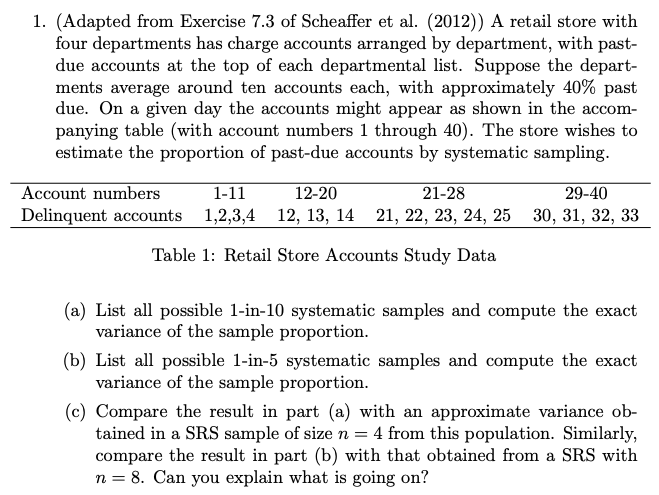
\includegraphics[width = 15cm]{img/Q1.png}
    %\caption{Section 6.1 Q8}
    %\label{fig:figure1label}
\end{figure}

~\

\subsection{(a)}
We need to fix the starting point, when start at 1: the number of deliquent accounts is 3, 
the sample proportion is $\frac{3}{4}.$ 

When start at 2: the number of deliquent accounts is 4. The sample proportion is $1.$

When start at 3: the number of deliquent accounts is 4. The sample proportion is $1.$ 

When start at 4: the number of deliquent accounts is 3. The sample proportion is $\frac{3}{4}.$ 

When start at 5: the number of deliquent accounts is 1. The sample proportion is $\frac{1}{4}.$ 

When start at 6: the number of deliquent accounts is 0. The sample proportion is $0.$ 

When start at 7: the number of deliquent accounts is 0. The sample proportion is $0.$ 

When start at 8: the number of deliquent accounts is 0. The sample proportion is $0.$ 

When start at 9: the number of deliquent accounts is 0. The sample proportion is $0.$ 

When start at 10: the number of deliquent accounts is 1. The sample proportion is $\frac{1}{4}.$ 

Therefore the exact variance of sample proportion is $0.165.$

\subsection{(b)}
When start at 1: the number of deliquent accounts is 3. The sample proportion is $0.375.$

When start at 2: the number of deliquent accounts is 4. The sample proportion is $0.5.$

When start at 3: the number of deliquent accounts is 4. The sample proportion is $0.5.$

When start at 4: the number of deliquent accounts is 3. The sample proportion is $0.375.$

When start at 5: the number of deliquent accounts is 2. The sample proportion is $0.25.$

Hence the exact variance of sample proportion is $8.75\times 10^{-3}.$

\subsection{(c)}
Using the formulae $$Var(\hat{p})=\frac{N-n}{N-1}p(1-p).$$

And we have $p=0.4, N=40,$ therefore $Var(\hat{p})=0.0554.$

For $n=8$, $Var(\hat{p})=0.0246.$

When n=4, SRS's variance is smaller and when n=8, SRS's is larger.

Because when $n=4,$ the ICC (intracluster coorelation coefficient) is tend to be larger, because
ICC represents how things are similar inside a cluster. Therefore $Var(\hat{p})$ tends to be 
underestimating.

And when $n=8$, the ICC is smaller, then $Var(\hat{p})$ tends to be overestimating.

\newpage
\section{Q2}
\begin{figure}[htp]
    \centering % 图片居中
    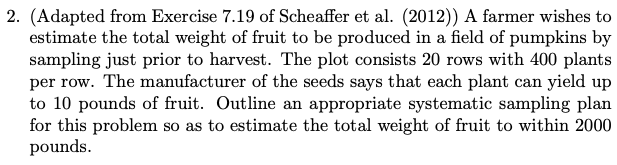
\includegraphics[width = 15cm]{img/Q2.png}
    %\caption{Section 6.1 Q8}
    %\label{fig:figure1label}
\end{figure}

~\ 

Note that we can regard every plant's condition is the same. Therefore we can apply the 
formulae from SRS: $$n=\frac{1}{\frac{1}{N} + 
\frac{d^2}{N^2v^2z_{1-\frac{\alpha}{2}}^2}(1-\frac{1}{N})}.$$

The $v$ is the "pre-sample estimate". We calculate it by Range Rule of Thumb, which is 
we calculate the variance by range divide by 4: $v=(10-0)/4=2.5$

And we have $N=20\times 400 = 8000,$ $d=2000,$ $z_{1-\frac{\alpha}{2}}=z_{0.975}=1.96.$

Hence we can calculate $n=366.6016.$ Therefore we take $n=367.$

And by $8000/366.6=21.8221.$ So take $k$ (the stepsize) be 21. 

To summarize, we should perform a 1-in-21 systematic sampling.


\newpage
\section{Q3}
\begin{figure}[htp]
     % 图片居中
    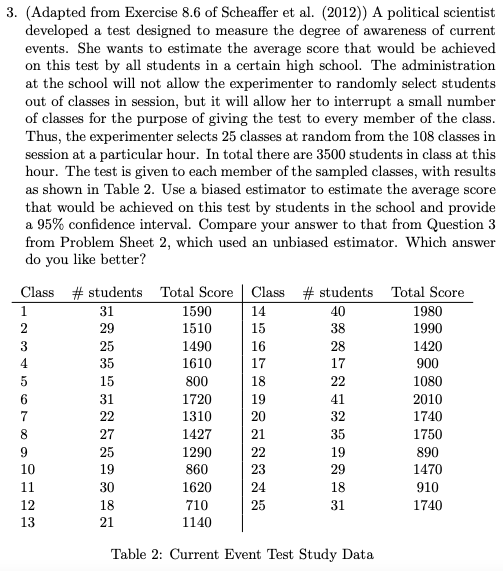
\includegraphics[width = 14cm]{img/Q3.png}
    %\caption{Section 6.1 Q8}
    %\label{fig:figure1label}
\end{figure}

~\ 

For sure we will apply the "using auxiliary data" method.

Define $X_i$ is the number of students in sampled class $i$. (E.g. 
$X_1=31$.)

Define $Y_i$ is the total score of sampled class $i$. (E.g. $Y_1=1590.$)

Hence $\bar{Y}=\frac{1}{25}\sum_{i=1}^{25}Y_i=1398.28.$ And 
$\bar{X}=\frac{1}{25}\sum_{i=1}^{25}X_i=27.12.$ 
Then $$\hat{R}=\frac{\bar{Y}}{\bar{X}}=51.5590.$$

Hence $\hat{\mu}=51.5590.$

Then using the formulae 
$\widehat{Var(\hat{\mu})}=\frac{N}{M^2}(N-n)\frac{1}{n}\hat{\sigma_r^{2}}.$ 
Where $\hat{\sigma_r^{2}}=10808.7251.$

We can gain that $\widehat{Var(\hat{\mu})}=0.3164.$

Therefore, an 95\% C.I. can be $(51.5590 \pm t_{24,0.975}\sqrt{0.3164}~)=(50.3981,52.7199).$

Recall that the result from Problem Set 2 is $(43,147 \pm 4.3081).$

I prefer the biased approach, because this has a much smaller variance.

\newpage
\section{Q4}
\begin{figure}[htp]
     % 图片居中
    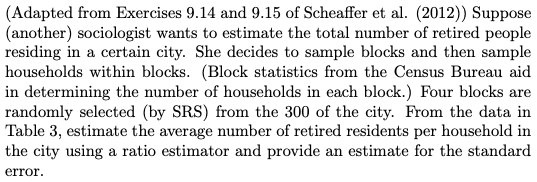
\includegraphics[width = 14cm]{img/Q4.png}
    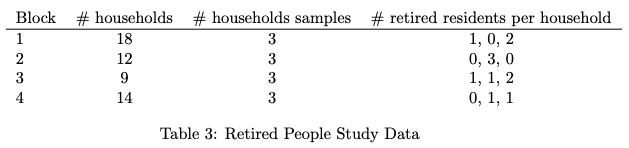
\includegraphics[width = 14cm]{img/Q3(2).png}
    %\caption{Section 6.1 Q8}
    %\label{fig:figure1label}
\end{figure}


~\ 

Make it clear that we want to estimate $\mu$ the average number of retired residents per household.

Before beginning, we need to make sure that $n=4, N=300.$

We are in the sampling method of "ratio estimation and two-stage cluster sampling."

And adopting an point estimate of $\mu$ is 
$$\hat{\mu}=\frac{\sum_{i=1}^n M_i\bar{Y_i}}{\sum_{i=1}^{n}M_i}=\frac{ 18*1+12*1+9*(4/3)+14*(2/3)  }{ 18+12+9+14 }=0.9686.$$

And we then need to determine 
$$\widehat{Var(\hat{\mu})}=\frac{1}{M^2}N(N-n)\frac{1}{n}\hat{\sigma_r^2}+\frac{1}{M^2}\frac{N}{n}\sum_{i=1}^n M_i(M_i-m_i)\frac{1}{m_i}\hat{\sigma_i}^2.$$

And $\hat{\sigma_r}^2=\frac{1}{n-1}\sum_{i=1}^n(\hat{Y_i}-M_i \hat{\mu_r})=9.7017.$

And $\hat{\sigma_i}^2$'s are variance inside each cluster i. 
Hence the 4 values are 1, 3, 0.3333, 0.3333.

And we do not have $M$, so we need to estimate 
$\hat{M}=\frac{N}{n}\sum_{i=1}^n M_i=3975.$

Hence $\widehat{Var(\hat{\mu})}=0.0136+1.0495\times 10^3=0.01465=0.1210^2.$

Therefore the standard error is $0.1210.$

\newpage
\section{Q5}
\begin{figure}[htp]
     % 图片居中
    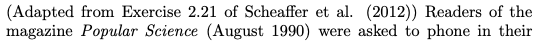
\includegraphics[width = 14cm]{img/Q5(1).png}
    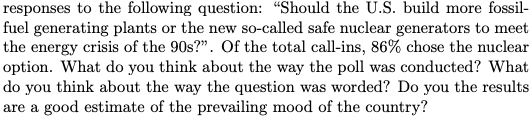
\includegraphics[width = 14cm]{img/Q5(2).png}
    %\caption{Section 6.1 Q8}
    %\label{fig:figure1label}
\end{figure}

Note that the survey is conducted in a way that without any sampling. 
Hence they just let readers to state their response voluntarily. 

And in the wording of the question, the "so-called safe" is not needed. This implies that
the question is not balanced.

Hence I don't think the results are a good estimate of prevailing mood of the country. If
one wants to get good estimate of prevailing mood of the country, one needs to sample the 
country by adopting some proper sampling method.

\newpage
\section{Q6}
\begin{figure}[htp]
     % 图片居中
    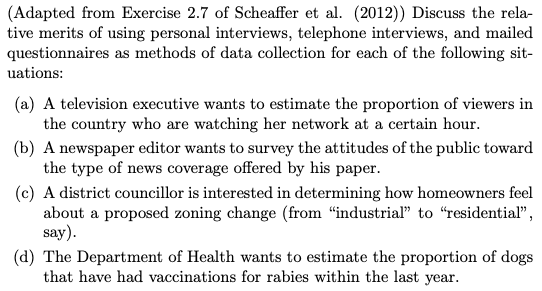
\includegraphics[width = 14cm]{img/Q6.png}
    %\caption{Section 6.1 Q8}
    %\label{fig:figure1label}
\end{figure}

\subsection{(a)}
Telephone interview is a feasible way to conduct the survey. Because the pool to be sampled 
is the whole country, and the survey needs to be conducted soon after the TV programme starts.

\subsection{(b)}
Suppose the "public" means the readers (subscriber) of his paper, 
then since the paper company already has the frame of those readers, then mailed questionnaires
with small reward is good.

\subsection{(c)}
I think the councillor should have a frame, since he can adopt the mailed questionnaires/
personal interview method. Since the problem seems like cannot be discussed through a simple
telephone call.


\subsection{(d)}
Personal interview. Because in this situation, the survey is officially conducted, 
I suppose the Department of Health has a frame of registration institutes of pet hospitals, etc..

So there are many certificates or documents (e.g. the registration documents of dogs, etc.)
needed to be checked. In this sense, telephone and mailed questionnaires are not that proper.

If the Department can assure the document and certificates problem remotely, then telephone
interviews /mailed questionnaires are also feasible.


\newpage
\section{Q7}
\begin{figure}[htp]
     % 图片居中
    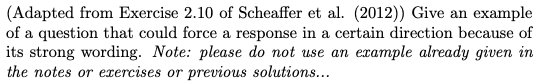
\includegraphics[width = 14cm]{img/Q7.png}
    %\caption{Section 6.1 Q8}
    %\label{fig:figure1label}
\end{figure}

"Do you for or against the execution of Lantau Tomorrow Plan of Hong Kong government?" comparing with 
"Do you for or against the execution of Lantau Tomorrow Plan at any cost?"


\section{Q8}
\begin{figure}[htp]
     % 图片居中
    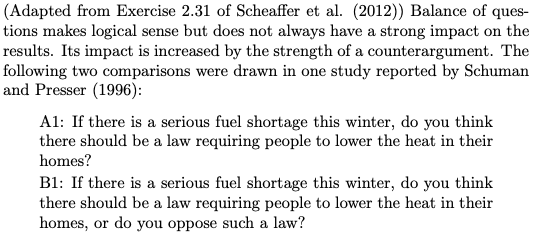
\includegraphics[width = 14cm]{img/Q8(1).png}
    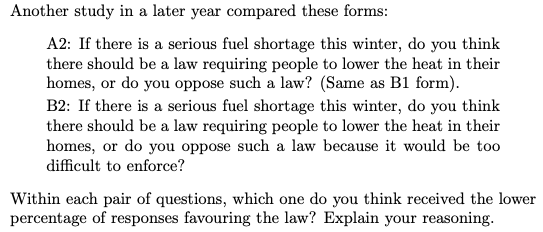
\includegraphics[width = 14cm]{img/Q8(2).png}
    %\caption{Section 6.1 Q8}
    %\label{fig:figure1label}
\end{figure}

In the A1B1 pair, the B1.

Because in A1B1 pair, because B1 reminds the respondents of a negative attitude.
Hence B1 is expected to have a lower percentage of favouring the law. And A1 is not as balanced as B1.

In the A2B2 pair, I cannot do a confident guess.

It is proper to say A2 will have a lower percentage, because B2 only include one 
possibility of opposing the law, while there are many other reasons to object the law.

But it is also reasonable to expect that B2 will have a lower percentage.
Because A2 does not give the respondents a concrete and vivid situation (argument), 
or the feeling of difficuility of enforcing the law. 
While the B2 gives a vivid situation of hindering the law's enforcing. 

Hence I cannot make a confident guess.



\end{document}
